%%%%%%%%%%%%%%%%%%%%%%%%%%%%%%%%%%%%%%%%%
% CN2 Labreport template
%
% License:
% CC BY-NC-SA 3.0 (http://creativecommons.org/licenses/by-nc-sa/3.0/)
%
%%%%%%%%%%%%%%%%%%%%%%%%%%%%%%%%%%%%%%%%%

\documentclass[parskip=full]{scrartcl}

\usepackage{siunitx}  % Provides the \SI{}{} command for typesetting SI units
\usepackage{graphicx} % Required for the inclusion of images
\usepackage{booktabs} % nicer tables
\usepackage[noabbrev]{cleveref} % automatic references
\usepackage{listings} % typeset code

\crefname{lstlisting}{listing}{listings} % for referencing code
\Crefname{lstlisting}{Listing}{Listings} % for referencing code

\usepackage[headsepline]{scrlayer-scrpage} % header
\ohead{Group 08} % right part of header
\ihead{Assignment 2} % left part of header

\lstset{basicstyle=\ttfamily} % monospaced font in listing

\usepackage{lstautogobble}  % Fix relative indenting
\usepackage{color}          % Code coloring
\usepackage{zi4}            % Nice font

\definecolor{bluekeywords}{rgb}{0.13, 0.13, 1}
\definecolor{greencomments}{rgb}{0, 0.5, 0}
\definecolor{redstrings}{rgb}{0.9, 0, 0}
\definecolor{graynumbers}{rgb}{0.5, 0.5, 0.5}

\usepackage{listings}
\lstset{
    autogobble,
    columns=fullflexible,
    showspaces=false,
    showtabs=false,
    breaklines=true,
    showstringspaces=false,
    breakatwhitespace=true,
    escapeinside={(*@}{@*)},
    commentstyle=\color{greencomments},
    keywordstyle=\color{bluekeywords},
    stringstyle=\color{redstrings},
    numberstyle=\color{graynumbers},
    basicstyle=\ttfamily\footnotesize,
    frame=l,
    framesep=12pt,
    xleftmargin=12pt,
    tabsize=4,
    captionpos=b
}


%----------------------------------------------------------------------------------------
%	DOCUMENT INFORMATION
%----------------------------------------------------------------------------------------

\begin{document}
\begin{titlepage}
    \centering
    \vspace*{2cm}
    {\Huge \textbf{Communication Networks 2}}\\
    SS 2017\\
    \vspace*{1cm}
    {\Large Assignment 2}
    \\\vspace*{3cm}
    {\Large \textbf{Group 08}}\\
    \vspace*{1cm}
    {\large 
        \begin{tabular}{l c c}
            Name & Mat.Nummer \\ \hline
            Constantin SCHIEBER & 01228774 \\
            Andreas HIRTENLEHNER & 01327273
        \end{tabular}
    }
    \\\vspace*{7cm}
    \today
\end{titlepage}

%----------------------------------------------------------------------------------------
%	SECTION 1
%----------------------------------------------------------------------------------------
\section{Description of the Solution}
Linphone was used and configured to register with the provided SIP Registrar (Figure \ref{fig:registerLinphone}).
The provided SIP identity and password were used (\texttt{sip:cn\_08@cn2lab.cn.tuwien.ac.aut}) for this.
\begin{figure}[ht]
    \centering
   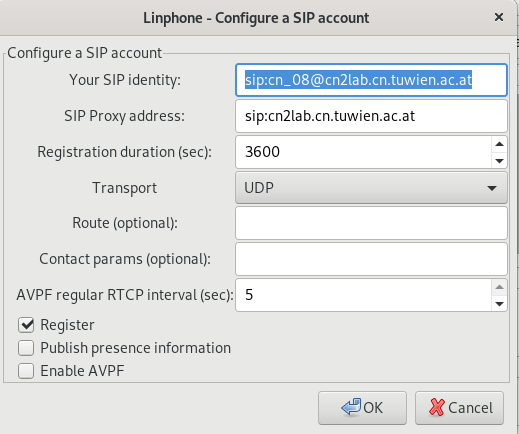
\includegraphics[width=0.5\textwidth]{images/linphoneSettings.png} 
    \caption{Setup of the Linphone client}
    \label{fig:registerLinphone}
\end{figure}

\subsection{Secret Message to the Registrar}
A Wireshark log was created to detect the secret message to the registrar.
A filter to \texttt{SIP} was set to observe the communication between the Registrar and our client.
We look for registration operations which enable the server to know the location of our client.
For this purpose, REGISTER messages are exchanged in a regular interval and the Registrar associates our SIP identity with our currently used machine (for a detailed description refer to RFC 3261, p. 16 and the lecture slides CN2-05-SIP, p. 103).
The \texttt{secret-message} field that is to be found is an unrecognised SIP header that does not conform to the standards of the protocol.
It is present in the header of \texttt{200 OK} messages that are sent by the server and has the value \texttt{Dohugiwiqi3}.
The secret message is therefore \texttt{Dohugiwiqi3}.
\begin{figure}[ht]
    \centering
   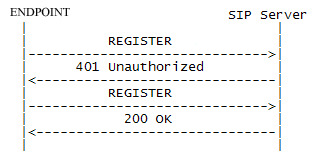
\includegraphics[width=0.5\textwidth]{images/sip_register_flow.jpg} 
    \caption{SIP Register Flow (https://www.voipmechanic.com/sip-call-example.htm)}
    \label{fig:sipRegisterFlow}
\end{figure}
\subsection{Discussion of Measured Network Parameters}
Factors that influence Quality of Service (QoS) include available bandwidth, latency, packet loss, packet delay variation, out-of-order delivery and rate of corrupted packets. 
With Wireshark, an analysis of lost packets, the delta between packets and the jitter is possible.

\begin{verbatim}
"Src addr","Src port","Dst addr","Dst port","SSRC","Payload","Packets","Lost","Max Delta (ms)","Max Jitter (ms)","Mean Jitter (ms)","Pb?"
"2001:1:6::face:b004","6002","2001:629:2600:a018:428d:5cff:fe10:2e9e","9078","0x86A4B38B","VP8","1553","0 (0.0%)","128,636775","10,739464","1,120582",""
"2001:1:6::face:b004","6000","2001:629:2600:a018:428d:5cff:fe10:2e9e","7078","0x4F6D67D8","opus","497","0 (0.0%)","43,523177","7,822404","4,946190",""
"2001:629:2600:a018:428d:5cff:fe10:2e9e","9078","2001:1:6::face:b004","6002","0x86A4B38B","VP8","1553","0 (0.0%)","136,734240","10,572953","0,349627",""
"2001:629:2600:a018:428d:5cff:fe10:2e9e","7078","2001:1:6::face:b004","6000","0x4F6D67D8","opus","497","0 (0.0%)","39,733756","5,741685","2,443102",""
\end{verbatim}

\subsection{Discussion of subjective QoS}
Subjective QoS:
\begin{itemize}
	\item Landline: 5 (very good quality)
	\item Satellite: 3 (slight knacking in audio, video freezing every 5s)
	\item Satellite Speex, MP4V-ES: bad quality, fragments in picture but no freezes, lag
	\item Landline Speex, MP4V-ES: No difference in quality
	\item Satellite H263-1998 PCMU: bad quality, smoother fragments in picture but no freezes, lag
	\item Landline H263-1998 PCMU: No difference in quality
\end{itemize}



%----------------------------------------------------------------------------------------
%	SECTION X
%---------------------------------------------------------------------------------------


%%%%%%%%%%%%%%%%%%%%%%%%%%%%%%%%%%%%%%%%%%%%%%%
\end{document}
